
\section{Ackley Function}
\label{sec:app:test:ackley}
  The \emph{Ackley function} is a widely used benchmark function in the field
  of optimization, particularly for evolutionary algorithms and swarm
  intelligence.
  Named after \textit{David H. Ackley} who introduced it in his 
  studies,\footnote{%
    Ackley, D. H. (1987) \enquote{A connectionist machine for genetic 
    hillclimbing}, Kluwer Academic Publishers, Boston MA.
  }
  the function is known for its property of having a large number of local
  minima while having one global minimum.
  This makes it particularly challenging for optimization algorithms that can
  easily get trapped in local minima.

  \begin{definition}[Ackley function]
    The \emph{Ackley function}, \(f: \mathbb{R}^2 \rightarrow \mathbb{R}\), is
    defined as:

    \begin{equation}
      \label{eq:app:test:ackley}
      f(x,\, y) = -20\, e^{-0.2 \sqrt{0.5 (x^2 + y^2)}}
        - e^{0.5\, [\cos(2 \pi x) + \cos(2\pi y)]} + e + 20
    \end{equation}

    where \(-5 \leq x\) and \(y \leq 5\).
  \end{definition}

  The function has a global minimum at \(f(0,\, 0) = 0\).
  A contour plot and a surface plot of the Ackley function are shown in
  \vref{fig:app:test:ackley}.

  \begin{figure}[ht!]
  \centering
  \begin{subfigure}[b]{0.4\textwidth}
    \centering
    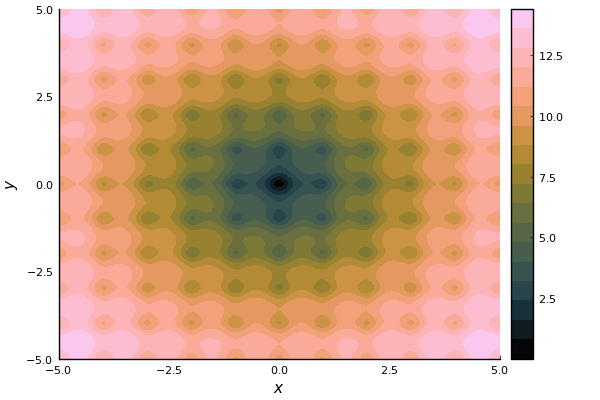
\includegraphics[width=\textwidth]{img/test_functions/ackley_contour.png}
  \end{subfigure}
  \begin{subfigure}[b]{0.4\textwidth}
    \centering
    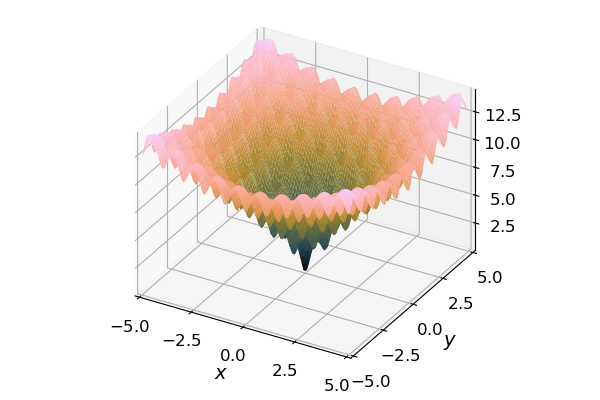
\includegraphics[width=\textwidth]{img/test_functions/ackley_surface.png}
  \end{subfigure}
  \caption{Ackley Function}
  \label{fig:app:test:ackley}
  \end{figure}